\chapter{Curvature of space}
\pagebreak[4]

\section{p82 - Exercise}
\begin{tcolorbox}
Explain why the surfaces of an ordinary cylinder and an ordinary cone are to be regarded as "flat" in the sense of our definition.
\end{tcolorbox}
The reason is because those surfaces can be "unwrapped" like the figure below shows. 
\begin{figure}[h]
%\centering
\begin{minipage}[t]{.4\textwidth}
%\centering
\vspace{0pt}
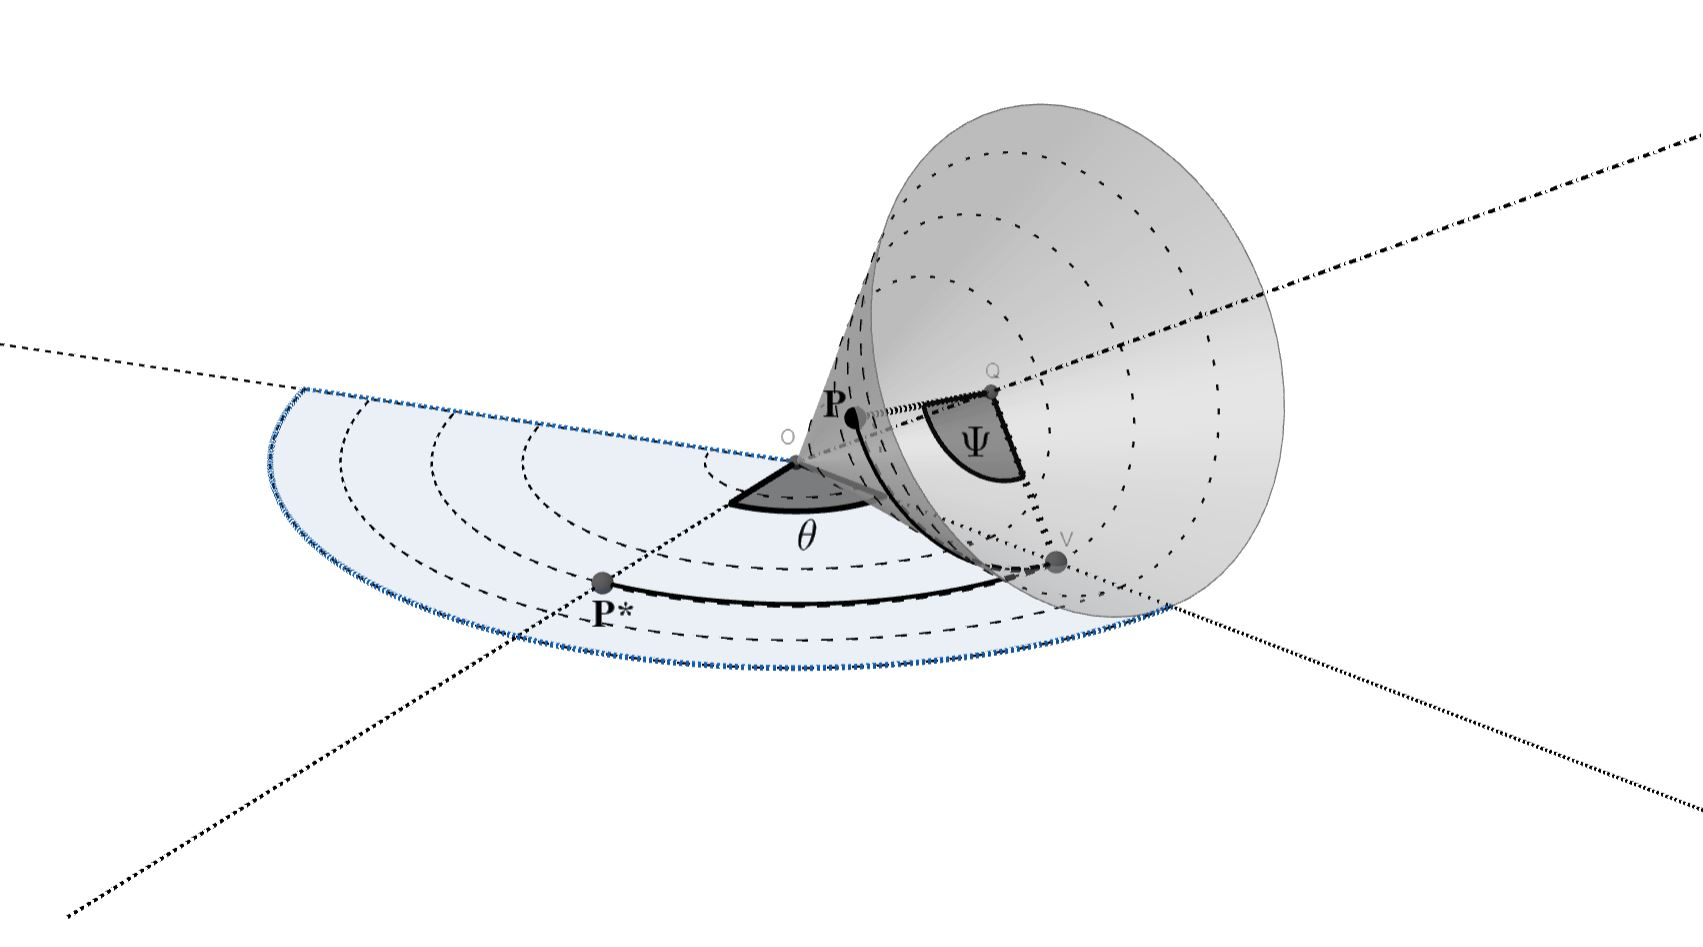
\includegraphics[scale=.5]{Conemapping.jpg}
\end{minipage}\hfill
\end{figure}\\
For the cone, we can for each point $\ P $ on the cone, lying on a distance $\ r $ from the apex and making an angle $\Psi $,  associate on a plane,  a  point $ P^* $ lying at the same  distance $ r $ from the apex, taken as origin for the coordinate system, and making an angle $\theta =  k\Psi $ with $ k $ a constant depending on the shape of the cone. This pair of coordinates are polar coordinates with $ r \in (-\infty, + \infty)$ and $\theta \in [0, 2k\pi)$. 
The same reasoning can be applied to a cylinder which is a cone with the apex at $\infty$. In that case the coordinate system becomes a Cartesian coordinate system. \\
As a continuous mapping exist from polar to orthogonal Cartesian coordinates both  coordinate system can be written under the required form (3.101) and so can be called "flat".

$$\blacklozenge$$
\newpage

\section{p83 - Exercise}
\begin{tcolorbox}
What are the values of $R^s_{.rmn}$ in an Euclidean plane, the coordinates being rectangular Cartesians? Deduce the values of the components of this tensor for polar coordinates from its tensor character, or else by direct calculation.
\end{tcolorbox}
See 2.64 page 139 (exercise 18).
$$\blacklozenge$$
\newpage

\section{p86 - Exercise}
\begin{tcolorbox}
Show that in a $V_2$ all the components of the covariant curvature tensor either vanish or are expressible in terms of $R_{1212}$.
\end{tcolorbox}
We have (3.115) and (3.116)
\begin{align}
\left \{ \begin{array}{l}
\ R_{rsmn} =  - R_{srmn}\\
\ R_{rsmn} =  - R_{rsnm}\\
\ R_{rsmn} =   R_{mnrs}\\
\ R_{rsmn} + R_{rmns}+R_{rnsm}=0
\end{array} \right.
\end{align}
It is clear from the two first identities that  in pairs $(rs)$ and $(mn)$ both indices have to be different when the tensor is not $0$. So we only have to consider $R_{1212}$,  $R_{1221}$, $R_{2112}$ and $R_{2121}$.\\
The two first  identities gives us:
\begin{align}
 R_{1221}= -R_{1212}\\
 R_{2112}= -R_{1212}\\
 R_{2121}= -R_{2112} = R_{1212}
\end{align}
The third identity does give us any additional information.
The fourth identity gives us only trivial statements:
\begin{align}
 R_{1212} + \underbrace{R_{1122}}_{=0}+\underbrace{R_{1221}}_{=- R_{1212} } = 0\\
 \underbrace{R_{1221}}_{=- R_{1212}} + R_{1212}+\underbrace{R_{1122}}_{=0 } = 0\\
 \underbrace{R_{2112}}_{=- R_{1212}} + \underbrace{R_{2121}}_{=R_{1212}}+\underbrace{R_{2211}}_{=0} = 0\\
 \underbrace{R_{2121}}_{= R_{1212}} + \underbrace{R_{2211}}_{=0}+\underbrace{R_{2112}}_{= -R_{1212}} = 0
\end{align}
$\textbf{Conclusion:}$\\
We get the identities (2), (3) and (4) in function of $R_{1212}$ and all vanish if $R_{1212} = 0$
$$\blacklozenge$$
\newpage

\section{p86-87 - clarification}
\begin{tcolorbox}
\textit{The number of independent components of the covariant curvature tensor in a space of N dimensions is} $$\frac{1}{12}N^2\left(N^2-1\right)$$
\end{tcolorbox}
We have (3.115) and (3.116)
\begin{align}
\left \{ \begin{array}{l}
R_{rsmn} =  - R_{srmn}\\
R_{rsmn} =  - R_{rsnm}\\
R_{rsmn} =   R_{mnrs}\\
R_{rsmn} + R_{rmns}+R_{rnsm}=0
\end{array}\right.
\end{align}
It is clear from the two first identities that  in the tuple $(rs)$ and $(mn)$ both indices have to be different when the component is not $0$. So we only have to consider the component with the pair of tuples $(r,s)$ and $m,n)$ with $r \neq s$ and $m \neq n$.
For the tuple $(r,s)$ we have $N$ possibilities to draw an index for $r$ but for $s$ only $N-1$ indices remain as $r \neq s$. So for the tuple $(r,s)$ we get $N(N-1)$ possibilities. But note by the first identity $R_{rsmn} =  - R_{srmn}$ that we only have to consider the half of this quantity as once we have chosen a tuple $(r,s)$ we also know  the component for the tuple $(s,r)$. So the total number of possibilities we have for  $(r,s)$ is $M = \half N(N-1)$. The same yields for the tuple $(mn)$. So, we get in total $M^2$ possibilities according to the two first identities.\\
The third identity $R_{rsmn} =   R_{mnrs}$ puts an extra constraint on the number of possibilities as we have to subtract from $M^2$ the number of possibilities covered by this third identity. Note that, once we have chosen a tuple $(rs)$ we have to exclude the tuple $(m,n) =  (r,s)$ as the identity $R_{rsrs} =   R_{rsrs}$ becomes trivial.. So for the first tuple we have $M$ possibilities, but once chosen, only $M-1$ remain for the second tuple. So we get $M(M-1)$ possibilities. But, again we only have to take half of these possibilities as the identities $R_{rsmn} =   R_{mnrs}$ and $ R_{mnrs} = R_{rsmn}$ are equivalent.\\
So the total number of possibilities reduces to $$ M^2 - \half M(M-1) \quad \text{with} \quad M=\half N(N-1) $$
What about the fourth identity $$R_{rsmn} + R_{rmns}+R_{rnsm}=0$$
First we note that this identity implies that all indices are different as it becomes trivial in the other cases. This is a consequence of the first 3 identities. Indeed, we know already that
\begin{align}
\left \{ \begin{array}{l}
\ r \neq s\\
\ m \neq n\\
\ (r,s) \neq (m,n)\\
\end{array} \right.
\end{align}
Let's consider the following cases
\begin{align}
\left \{ \begin{array}{llll}
\ r = m&\rightarrow m\neq s \  m\neq n \ r\neq n&\rightarrow & R_{rsrn} + \underbrace{R_{rrns}}_{=0}+\underbrace{R_{rnsr}}_{= -R_{rnrs}= -R_{rsrn}}=0\\
\ r = n&\rightarrow n\neq s \  m\neq n \ r\neq s&\rightarrow & R_{rsmr} + \underbrace{R_{rmrs}}_{= -R_{mrrs}= -R_{rsmr}}+\underbrace{R_{rrsm}}_{=0}=0\\
\ s = m&\rightarrow m\neq r \  n\neq s \ r\neq s&\rightarrow & R_{rssn} + \underbrace{R_{rsns}}_{= -R_{rssn}}+\underbrace{R_{rnss}}_{=0}=0\\
\ s = n&\rightarrow r\neq s \  m\neq s \ m\neq n&\rightarrow & R_{rsms} + \underbrace{R_{rmss}}_{=0}+\underbrace{R_{rssm}}_{= -R_{rsms}}=0
\end{array} \right.
\end{align}
So indeed, once two indices are equal, the fourth identity becomes trivial and does not put extra constraints to the number of possibilities. For the tuple $(r,s,m,n)$ we have $N$ possibilities to draw an index for $r$, for $s$ only $N-1$, for $m$ only $N-2$ and for $n$ only $N-3$ indices remain as $r \neq s\neq m\neq n$. The maximum number of constraint generated by the fourth identity is thus $$N(N-1)(N-2)(N-3)$$
But here again double counts occur. Indeed the fourth identity is true for the $6$ tuples $$(rsmn),(rmsn) ,(rmns),(rsnm),(rnsm),(rnms)$$ as first entry    in the identity. The same reasoning is valid for the tuples $(n...), \ (s...) \ (m...) $. \\So in total we get $6\times4 = 24$ equivalent identities and the number of constraints generated by the fourth identity reduces to  $$\frac{1}{24}N(N-1)(N-2)(N-3)$$
Note that this number of constraints vanish for $N \leq 3$.\\
Putting it all together the number of independent components of $R_{rsmn}$ becomes
\begin{align}
\mho &= M^2 - \half M(M-1)-\frac{1}{24}N(N-1)(N-2)(N-3)\\
&= \half M(M+1)-\frac{1}{24}N(N-1)(N-2)(N-3)\\
&= \frac{1}{8} N(N-1) \left(N(N-1)+2\right)-\frac{1}{24}N(N-1)(N-2)(N-3)\\
&= \frac{N}{24} \left( 3N^2-6N^2+9N-6-N^3+3N^2+3N^2-9N-2N+6 \right)\\
&= \frac{1}{12}N^2 \left( N^2-1\right)
\end{align}
$$\blacklozenge$$
\newpage
